\section{Hardware Aspects}

\subsection{Pipeline Components Overview and Generalities}

\begin{frame}{Technological types of graphics hardware implementations}
  \begin{itemize}
  \item Two commonly-used technologies, specific pros/cons:
  \end{itemize}

  \begin{center}
  \small
  \def\arraystretch{1.2}
  \begin{tabular}{l|c|c}
  & \textbf{Fixed-function} & \textbf{Programmable} \\
  \hline
  \textbf{Technology} & Circuit & Software \\
  \textbf{Source form} & HDL & Source code \\
  \textbf{Product form} & Silicon, bitstream & Firmware binaries \\
  \textbf{Implementation medium} & FPGA, ASIC, SoC block & DSP, custom ISA \\
  \textbf{Arithmetic} & Fixed-point & Fixed-point, floating point \\
  \textbf{Clock rate} & Low & High \\
  \textbf{Pixel data access} & Queue (FIFO) & Memory \\
  \textbf{CPU control} & Direct registers & Mailbox \\
  \textbf{Die surface (tendency)} & High & Low \\
  \textbf{Reusability} & Low & High \\
  \hline
  \textbf{Example} & Allwinner SoCs Display Engine & TI TMS340 DSP \\
  \end{tabular}
  \end{center}
\end{frame}

\begin{frame}{Graphics memory and buffers}
  \begin{itemize}
  \item Pixel data is stored in memory buffers, called \textbf{framebuffers}
  \item Framebuffers live either on:
    \begin{itemize}
    \item \textbf{System memory}: shared with the rest of the system (e.g. SDRAM or SRAM)
    \item \textbf{Dedicated memory}: only for graphics (e.g. SGRAM)
    \end{itemize}
  \item Framebuffers that can be displayed are called \textbf{scanout framebuffers}\\
  \textit{hardware constraints don't always allow any framebuffer to be scanned out}
  \item CPU access to pixel data in dedicated memory is not always granted or easy!
  \item Graphics hardware \textbf{needs configuration} to interpret framebuffer pixel data\\
    \textit{pixel meta-data is rarely to never stored aside of the pixel data}
  \end{itemize}
\end{frame}

\begin{frame}{I/O with graphics hardware, pipelines}
  \begin{itemize}
  \item Graphics hardware is \textbf{I/O-based} and interacts with pixel data
  \item Pipeline elements have input-output abilities:
    \begin{itemize}
    \item \textbf{Source} components: \textbf{feed pixel data}: \textit{e.g. camera}
    \item \textbf{Sink} components: \textbf{grab pixel data}: \textit{e.g. display}
    \end{itemize}
  \item Some components are \textbf{both a source and a sink}: \textit{e.g. converters}
  \item Graphics components can be chained in \textbf{pipelines}\\
    \textit{Usually from a source-only element to a sink-only element}
  \end{itemize}

  \vspace{-2em}
  \begin{center}
  \includegraphics[width=0.7\textwidth]{slides/graphics-hardware/pipeline-sink-source.pdf}
  \end{center}
\end{frame}

\begin{frame}{Display hardware overview}
  \begin{itemize}
  \item \textbf{Stream pixel data} to a display device, via a display interface
  \item Internal pipeline with \textbf{multiple components}
  \item Generally \textbf{fixed-function} hardware, pipeline sink only
  \item Either \textbf{discrete} (video card) or \textbf{integrated}
  \item Connected to the CPU (and RAM) via a \textbf{high-speed bus}:\\
  \textit{e.g. AXI with ARM, ISA, PCI, AGP, PCI-e with x86}
  \end{itemize}~

  \begin{minipage}[t]{0.45\textwidth}
    \centering
    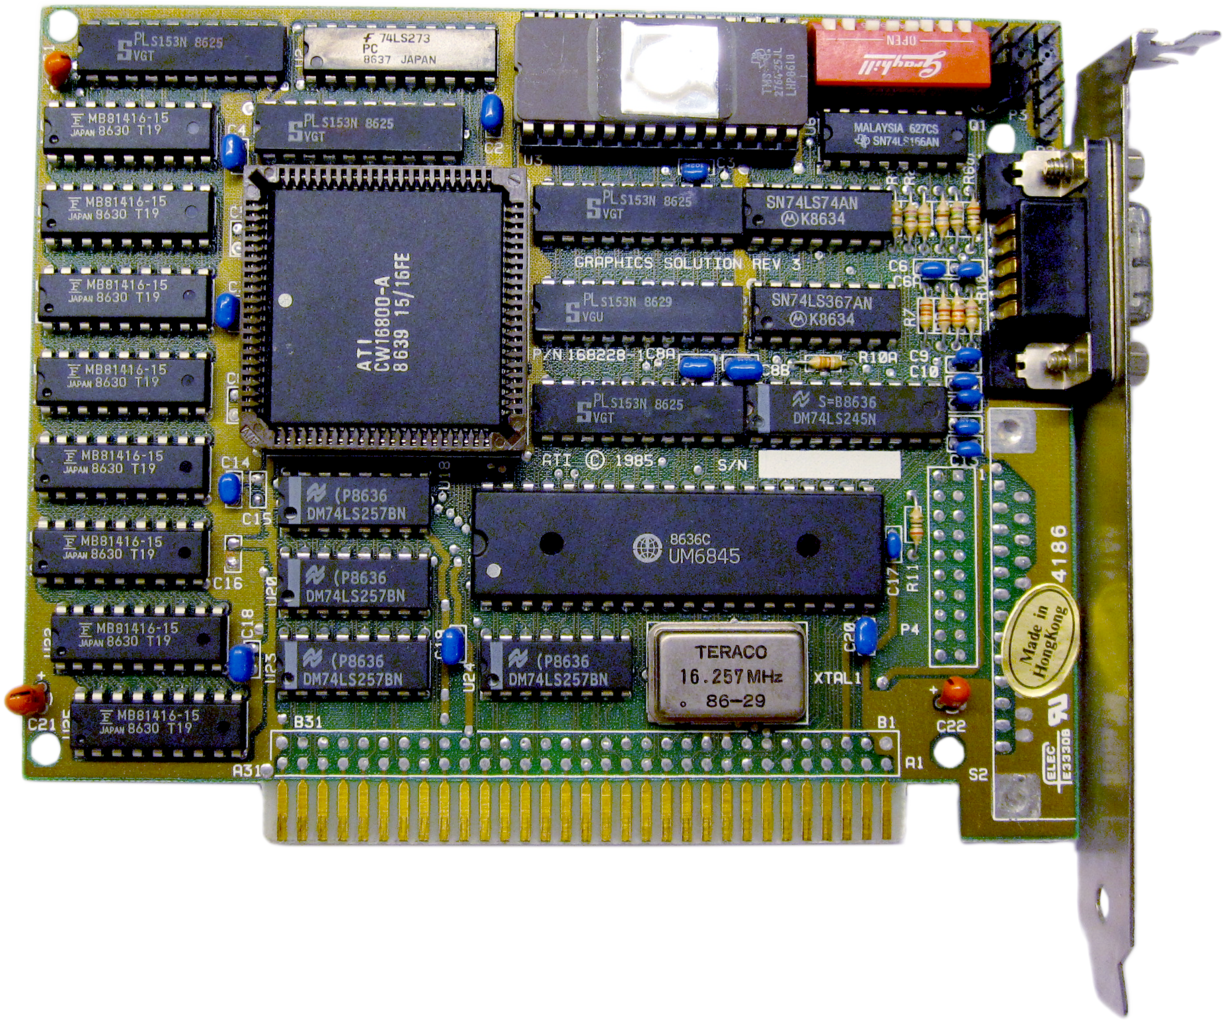
\includegraphics[height=7em]{slides/graphics-hardware/ati-hercules-1986.png}\\
    \textit{\small A 1986 Hercules discrete video card}
  \end{minipage}
  \hfill
  \begin{minipage}[t]{0.45\textwidth}
    \centering
    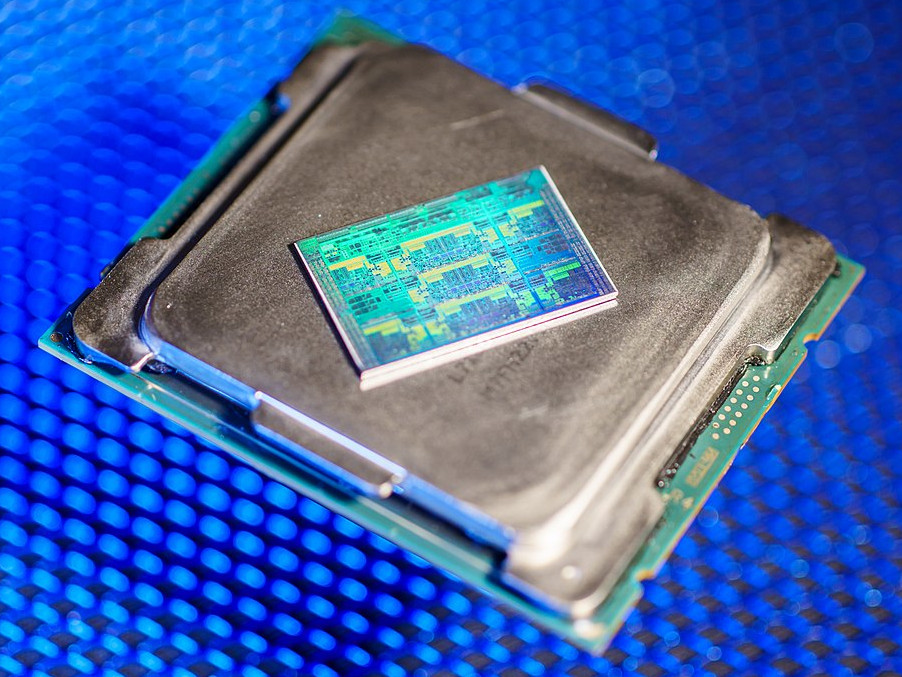
\includegraphics[height=7em]{slides/graphics-hardware/intel-skylake.jpg}\\
    \textit{\small An Intel processor with integrated graphics}
  \end{minipage}
\end{frame}

\begin{frame}{Common components of a display pipeline overview}
  \begin{center}
  \includegraphics[width=0.7\textwidth]{slides/graphics-hardware/display-pipe.pdf}
  \end{center}

  \begin{enumerate}
  \item \textbf{Framebuffers} where the pixel data is stored
  \item \textbf{Planes} that associate a framebuffer with its dimensions and position
  \item \textbf{CRTC} for pixel composition and streaming\\
  \textit{The CRTC terminology comes from the legacy Cathode-Ray Tube Controller}
  \item \textbf{Encoder} for meta-data addition and physical signal conversion
  \item \textbf{Connector} for video signal, display data channel (DDC), hotplug detection
  \item \textbf{Monitor} for decoding and displaying pixels (decoder and panel)
  \end{enumerate}
\end{frame}

\begin{frame}{Render hardware overview}
  \textbf{Rendering} hardware includes a wide range of aspects (usual cases below):
  \begin{itemize}
  \item \textbf{Basic} pixel processing:
  \begin{itemize}
    \item Common operations: pixel format, CSC, dithering, scaling, blitting and blending
    \item Fixed-function hardware, pipeline sink and source
  \end{itemize}
  \item \textbf{Complex} pixel processing:
  \begin{itemize}
    \item Defined by the application: any computable operation
    \item Programmable hardware (DSP), pipeline sink and source
  \end{itemize}
  \item \textbf{2D vector} drawing:
  \begin{itemize}
    \item Rasterisation from equations, parameters and data (e.g. points)
    \item Either fixed-function or programmable hardware (custom), pipeline source
  \end{itemize}
  \item \textbf{3D scene} rendering:
  \begin{itemize}
    \item Rasterisation from programs (shaders) and data (e.g. vertices, lines, triangles textures)
    \item Programmable hardware (GPU), pipeline source
  \end{itemize}
  \item Rendering can \textbf{always fallback} to general-purpose CPU operations
  \end{itemize}
\end{frame}

\begin{frame}{Video hardware overview}
  \textbf{Video-oriented} hardware comes in different forms (usual cases below):

  \begin{itemize}
  \item \textbf{Hardware video decoder} (VPU/video codec decoder)
  \begin{itemize}
    \item Decodes a video from compressed data (bitstream) to pixel frames
    \item Fixed-function hardware, pipeline source
  \end{itemize}
  \item \textbf{Hardware video encoder} (VPU/video codec encoder)
  \begin{itemize}
    \item Encodes a video from pixel frames to compressed data (bitstream)
    \item Fixed-function hardware, pipeline sink
  \end{itemize}
  \item \textbf{Camera sensors, video input, video broadcasting} (DVB)
  \begin{itemize}
    \item Receives/sends data in a given configuration from/to \textit{the outside}
    \item Can be compressed data (bitstream) or raw pixel data
    \item Fixed-function hardware, pipeline source
  \end{itemize}
  \end{itemize}~
\end{frame}

\begin{frame}{Building complex pipelines}

  \begin{itemize}
  \item Display, rendering and video elements are chained from source(s) to sink(s)
  \item On source-sink boundaries:
    \begin{itemize}
    \item Mutually-supported pixel format (or conversion)
    \item Mutually-accessible memory (or copy)
    \end{itemize}
  \item Target frame rate (\(fps\)) gives a time budget for pipeline traversal:
  \( t_0 + t_2 + t_4 + t_5 < fps^{-1},~ t_0 + t_3 < fps^{-1},~ t_1 + t_4 + t_5 < fps^{-1} \)
  \end{itemize}

  \begin{center}
  \includegraphics[width=0.7\textwidth]{slides/graphics-hardware/pipeline-complex.pdf}
  \end{center}

\end{frame}

\subsection{Display Hardware Specifics}

\begin{frame}{Visual display technologies generalities}
  \begin{itemize}
  \item Pixel data is pushed from the display interface to a visible surface\\
  \textit{using a dedicated controller on the display device}
  \item Pixels are split into 3 color cells (R-G-B)
  \item The human eye naturally merges light from the 3 cells
  \item Pixel frames are displayed as (physical) arrays of color cells
  \end{itemize}~

  \begin{minipage}[b]{0.45\textwidth}
    \centering
    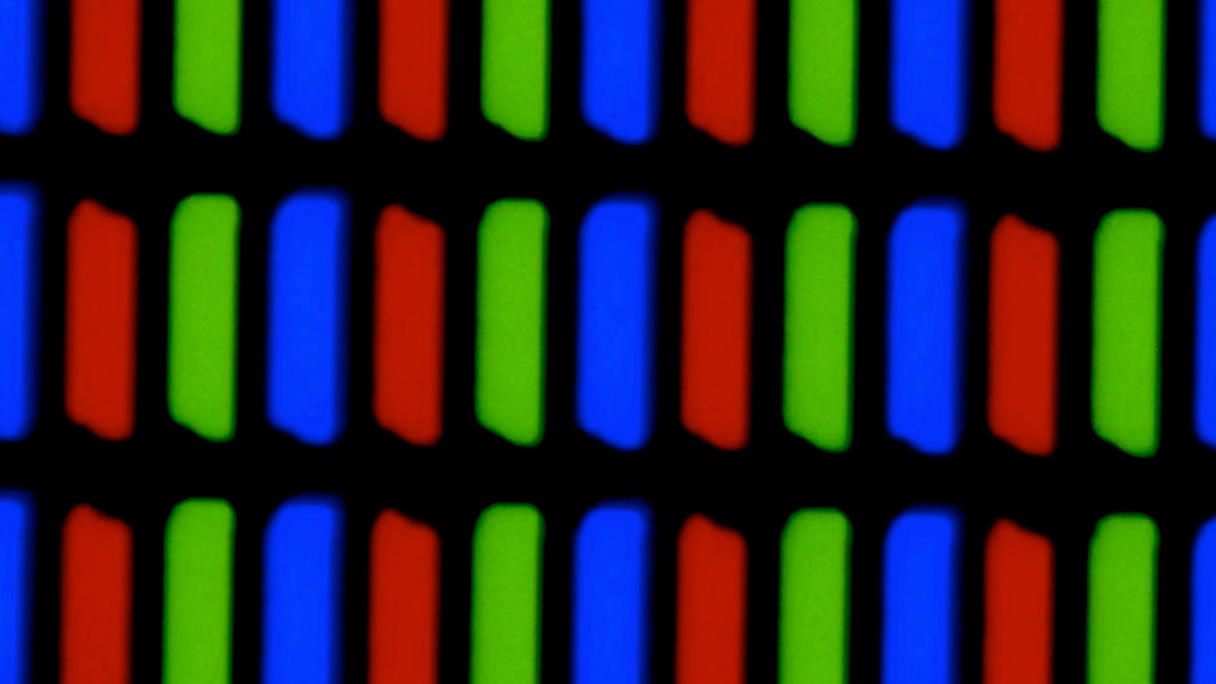
\includegraphics[height=6.5em]{slides/graphics-hardware/pixel-array.jpg}\\
    \textit{\small Pixel color cells on a LCD TN panel}
  \end{minipage}
  \hfill
  \begin{minipage}[b]{0.45\textwidth}
    \centering
    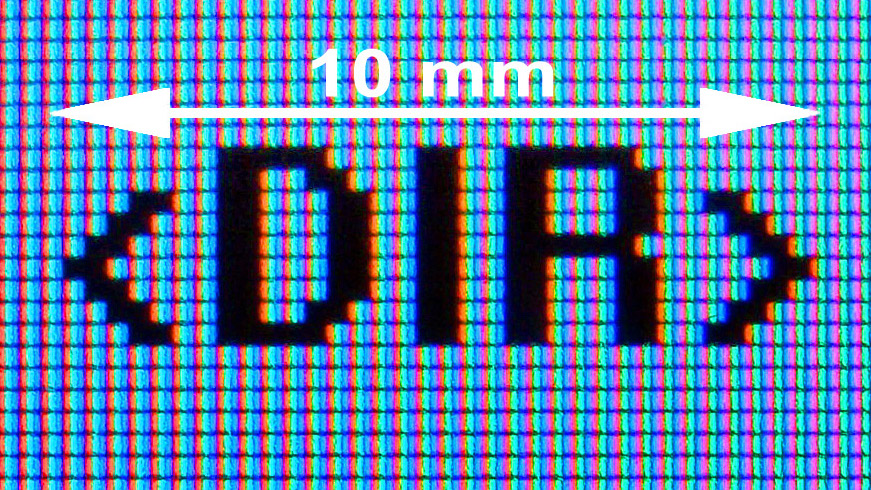
\includegraphics[height=6.5em]{slides/graphics-hardware/pixel-array-text.jpg}\\
    \textit{\small A pixel array displaying text}
  \end{minipage}
\end{frame}

\begin{frame}{CRT display technology}
  \begin{itemize}
  \item Color \textbf{cathode-ray tubes} (CRTs), since the 1950s:
    \begin{itemize}
    \item Using electron beams to excite a phosphorescent screen
    \item Beams are guided by magnetic deflection
    \item One beam for each color with increased intensity for increased luminosity
    \item High energy consumption
    \item High contrast, medium response time (\(1-10~\mu s\))
    \item Other issues: monitor size, burn-in (screensavers), remanent magnetic field (degaussing), high voltages and magnetic fields
    \end{itemize}
  \end{itemize}

  \begin{center}
  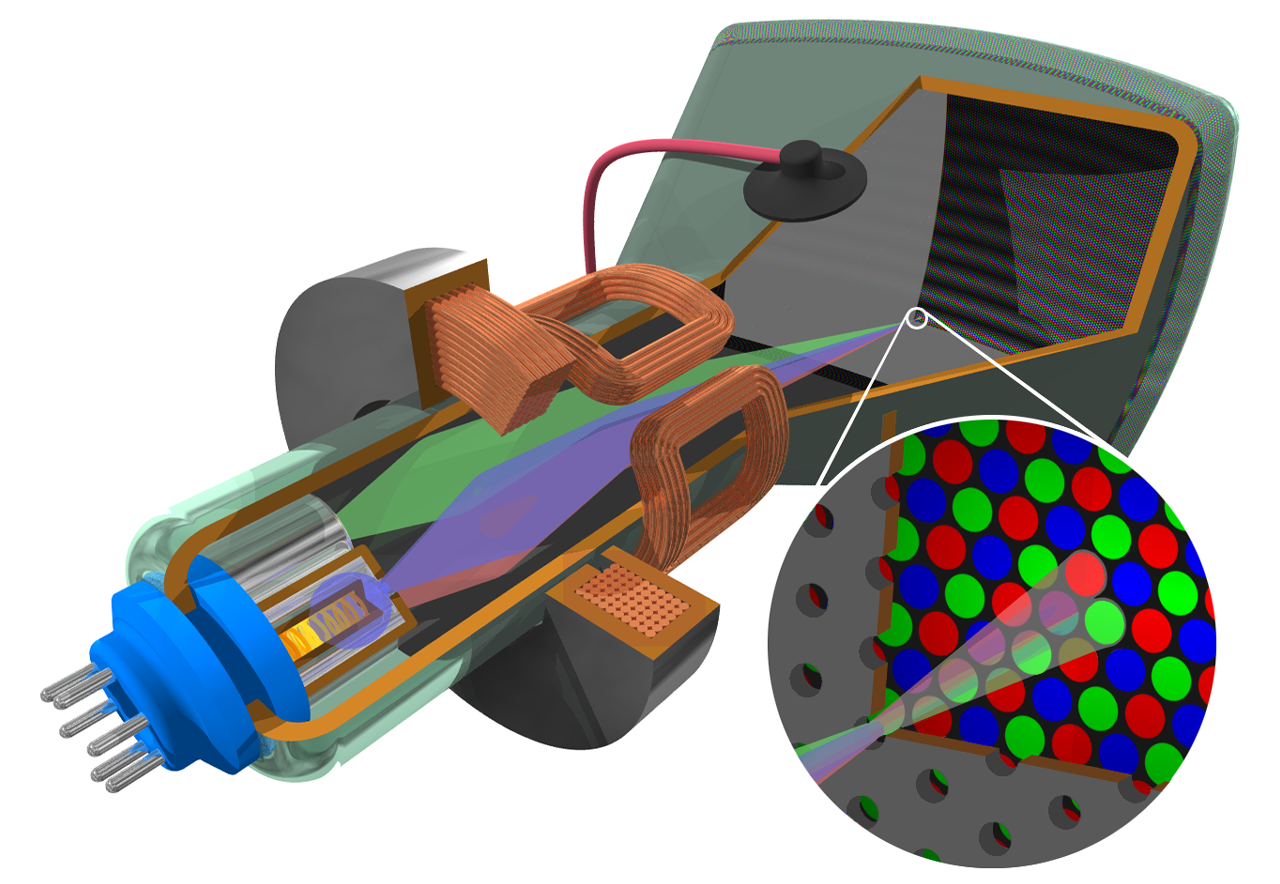
\includegraphics[height=8em]{slides/graphics-hardware/crt-color.png}
  \end{center}
\end{frame}

\begin{frame}{Plasma display panels technology}
  \begin{itemize}
  \item \textbf{Plasma display panels} (PDPs), since the 1990s-2000s:
    \begin{itemize}
    \item Using gas cells brought to plasma state to strike light-emitting phosphor
    \item Flat array of cells, scales to large surfaces
    \item Medium energy consumption (depends on luminance)
    \item Medium to low contrast, low response time (\(\leq 1~\mu s\))
    \item Other issues: burn-in
    \item Gradually being \textbf{deprecated} in favor of other flat-panel technologies
    \end{itemize}
  \end{itemize}
\end{frame}

\begin{frame}{LCD display technology}
  \begin{itemize}
  \item \textbf{Liquid crystal displays} (LCDs) using \textbf{Thin-film-transistors} (TFT):
    \begin{itemize}
    \item Using the electrically-controlled alignment of crystal structures to block light
    \item Does not emit light: needs an always-on backlight source (usually LEDs)
    \item Low energy consumption (depends on backlight)
    \item Medium to low contrast, high response time (\(1-10~ms\))
    \item \textbf{Twisted nematic} (TN): limited color quality and viewing angles, since the 1980s
    \item \textbf{In-plane switching} (IPS): improved color and viewing angles, since the 2000s
    \end{itemize}
  \end{itemize}

  \begin{center}
  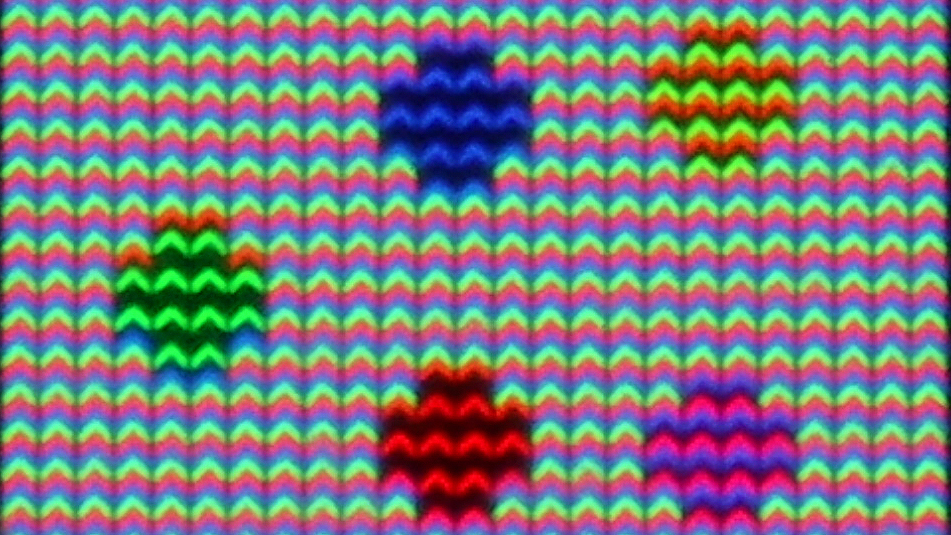
\includegraphics[height=6em]{slides/graphics-hardware/lcd-ips-shape.jpg}\\
  \textit{\small Chevron shapes that improve the viewing angle on IPS LCDs}
  \end{center}
\end{frame}

\begin{frame}{OLED display technology}
  \begin{itemize}
  \item \textbf{Organic light-emitting diodes} (OLEDs), since 2010:
    \begin{itemize}
    \item Using organic compounds (carbon-based) to emit light as R-G-B LEDs
    \item Allows flat and flexible surfaces, with a large viewing angle
    \item Low energy consumption
    \item Very high contrast, high response time (\(1-10~\mu s\))
    \item Issues: burn-in, independent cells aging, affected by UV light
    \item Rapidly becoming \textbf{very popular} and used
    \end{itemize}
  \end{itemize}

  \begin{center}
  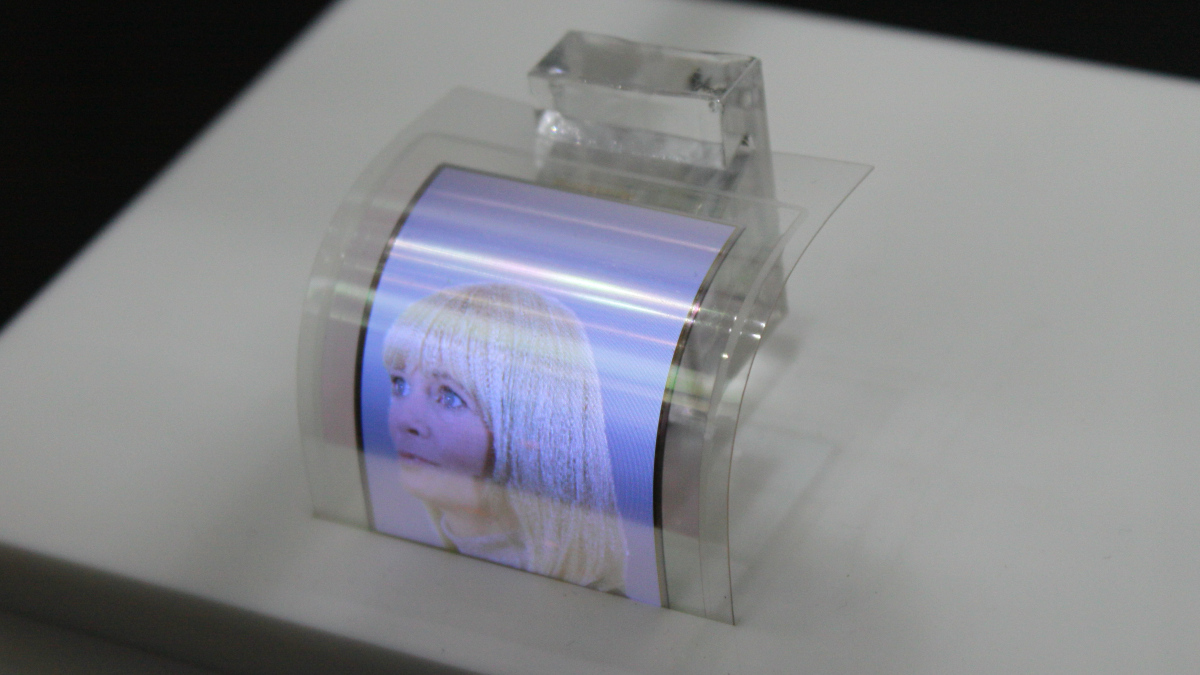
\includegraphics[height=8em]{slides/graphics-hardware/oled-display.jpg}\\
  \textit{\small A flexible OLED display panel}
  \end{center}
\end{frame}

\begin{frame}{EPD display technology}
  \begin{itemize}
  \item \textbf{Electrophoretic displays} (EPDs), since the 2000s:
    \begin{itemize}
    \item Using black and white electrically-charged particles in ink\\
    \textit{e.g. positive charge for black and negative for black}
    \item Electric fields attract one or the other color with current flow
    \textit{the particles stay in place after they were moved}
    \item Using incident light, does not emit light itself
    \item Very low consumption (only for changes)
    \item Low response time (\(1-10~\mu s\)) and ghosting
    \end{itemize}
  \end{itemize}~

  \begin{minipage}[b]{0.45\textwidth}
    \centering
    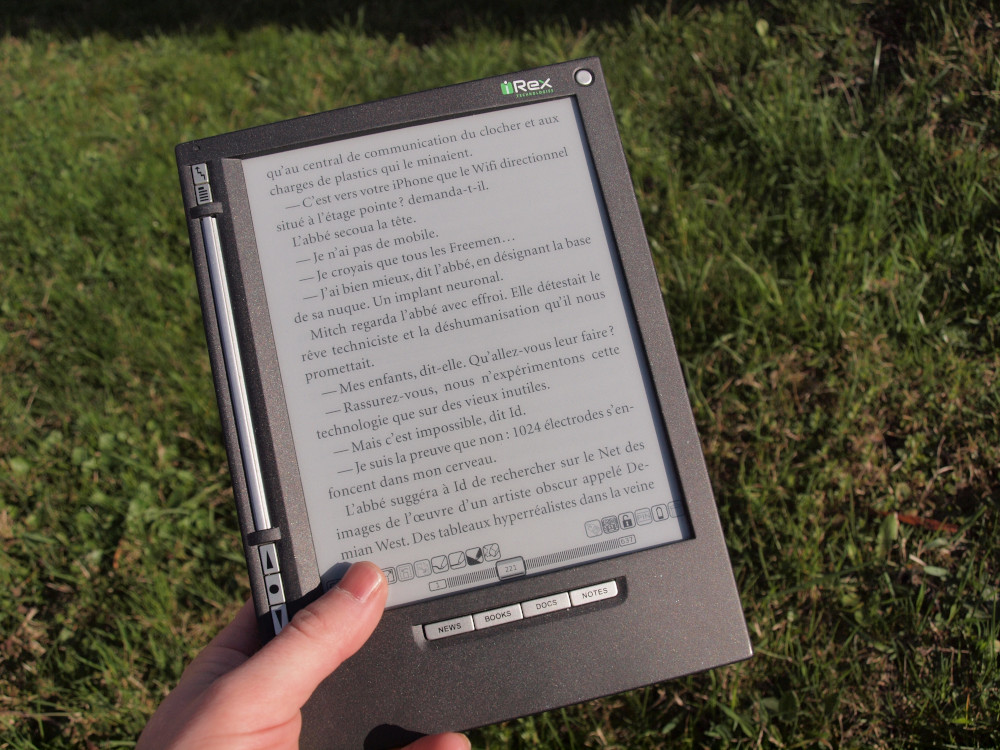
\includegraphics[height=6.5em]{slides/graphics-hardware/e-reader.jpg}\\
    \textit{\small An e-reader with an EPD display}
  \end{minipage}
  \hfill
  \begin{minipage}[b]{0.45\textwidth}
    \centering
    
\includegraphics[height=6.5em]{slides/graphics-hardware/epd-detail.jpg}\\
    \textit{\small Detail of an EPD display}
  \end{minipage}
\end{frame}

\begin{frame}{CRTs, refreshing and timings}
  \begin{itemize}
  \item CRTs need frequent refreshing or the picture fades out: \textbf{fixed refresh rate}
  \item An electron gun aims for pixels in \textbf{row-major/raster order}
  \begin{center}
  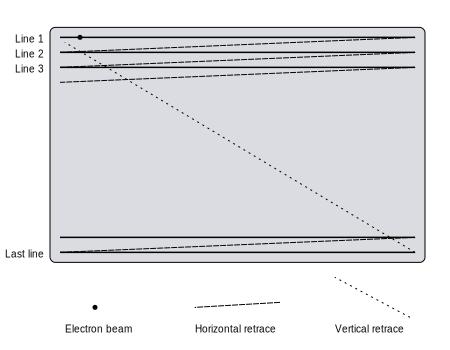
\includegraphics[height=8em]{slides/graphics-hardware/raster-scan.pdf}
  \end{center}
  \item Some \textbf{blank time} is needed to reposition the gun (horizontally and vertically)
  \item As a result, \textbf{specific timings} are needed for the signals to each CRT display
  \item For backwards compatibility with CRTs, \textbf{display timings are still necessary}
  \end{itemize}
\end{frame}

\begin{frame}{Display timings and modes}
  \begin{itemize}
  \item Timings coordinate how a frame is \textbf{transmitted to a display over time}
  \item Various signals are involved, synced to a \textbf{pixel clock} (time base)
  \item Display timings are split in a few stages (horizontal and vertical):
    \begin{enumerate}
    \item Sync pulse (vsync/hsync)
    \item Back porch (vbp/hbp)
    \item Active region (vactive/hactive)
    \item Front porch (vfp/hfp)
    \end{enumerate}
  \item Pixels are transmitted during the \textbf{horizontal active region} only
  \item A \textbf{display mode} groups timings, refresh rate and associated pixel clock rate
  \item Display signals are \textbf{generated by the CRTC}, according to the display mode
  \item Monitors usually support \textbf{multiple modes} (and dimensions)
  \end{itemize}
\end{frame}

\begin{frame}{Display timings and modes (illustrated)}
  \begin{center}
  \includegraphics[width=0.8\textwidth]{slides/graphics-hardware/display-timings.pdf}
  \end{center}

  \begin{itemize}
  \item The unit for horizontal stages is \textbf{one pixel clock period}
  \item The unit for vertical stages is \textbf{one line's duration}
  \end{itemize}
\end{frame}

\begin{frame}{Display timings and modes (panel example)}

  \begin{minipage}[b]{0.35\textwidth}
    \centering
    \vspace{2em}
    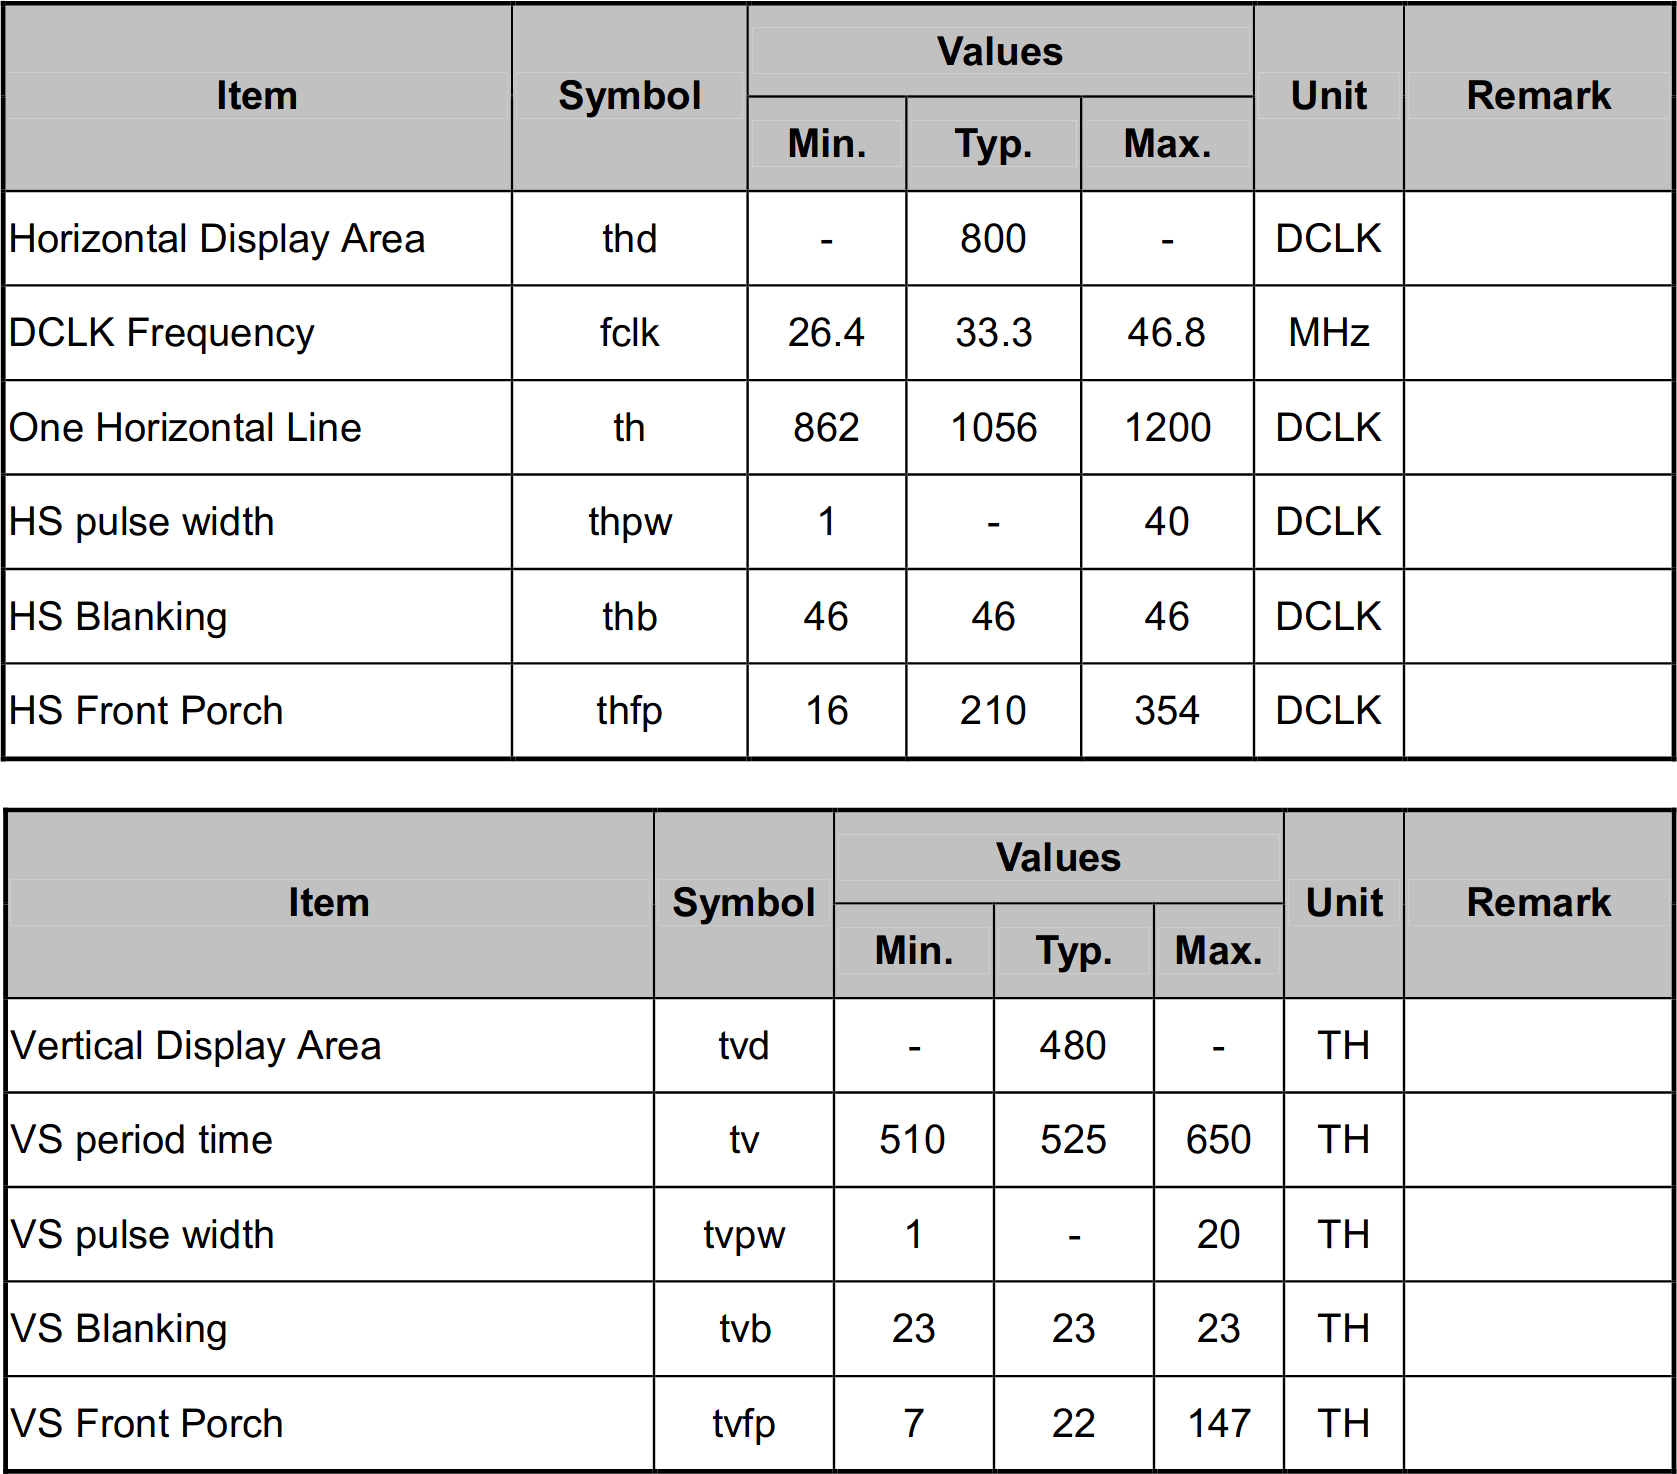
\includegraphics[width=\textwidth]{slides/graphics-hardware/timings-table.png}
    \textit{\small AT070TN94 panel datasheet}
    \vfill~
  \end{minipage}
  \hfill
  \begin{minipage}[b]{0.6\textwidth}
    \small
    \begin{itemize}
    \item \(hsync = thpw = 20 \in \llbracket 1;40 \rrbracket\)\\
    \(hbp = thb - thpw = 46 - 20 = 26\) (from diagram)\\
    \(hactive = thd = 800\)\\
    \(hfp = thfp = 210 \in \llbracket 16;354 \rrbracket\)\\
    \(htotal = hsync + hbp + hactive + hfp = 1056\)

    \item \(vsync = tvpw = 10 \in \llbracket 1;20 \rrbracket\)\\
    \(vbp = tvb - tvpw = 23 - 10 = 13\) (from diagram)\\
    \(vactive = tvd = 480\)\\
    \(vfp = tvfp = 22 \in \llbracket 7;147 \rrbracket\)\\
    \(vtotal = vsync + vbp + vactive + vfp = 525\)
    \item 1 frame takes: \(vtotal \times htotal = 554400~t_{clk}\)\\
    60 frames take: \(vtotal \times htotal \times 60 = 33264000~t_{clk}\)\\
    60 fps requires: \(f_{clk} \geq 33.264~MHz\)
    \end{itemize}
  \end{minipage}
  \vspace{0.5em}

  \begin{itemize}
  \item Panels usually support a \textbf{range of timings}
  \item The pixel clock rate is often \textbf{rounded} (refresh rate not always strictly respected)
  \end{itemize}

\end{frame}

\begin{frame}{Side-channel and identification}
  \begin{itemize}
  \item Monitor display connectors often come with a \textbf{Display Data Channel} (DDC)
    \begin{itemize}
    \item Side-bus to allow communication between host and display
    \item Usually based on I2C, quite slow (\(\approx 100~kHz\))
    \end{itemize}
  \item DDC provides access to the \textbf{Extended Display Identification Data} (EDID)
    \begin{itemize}
    \item Contains the list of supported modes in a standard format
    \item Usually stored in an EEPROM at I2C address \(0x50\)
    \end{itemize}
  \item Another common monitor signal is \textbf{Hotplug Detect} (HPD)
    \begin{itemize}
    \item Connected to a pin of the connector, asserted with a cable plugged
    \item Can be wired to an interrupt pin to detect connection changes
    \end{itemize}
  \item Direct panel interfaces (not monitors) usually lack DDC, EDID and HPD
    \begin{itemize}
      \item Panel is always considered connected
      \item Modes need to be known in advance
    \end{itemize}
  \end{itemize}
\end{frame}

\begin{frame}{Extra display interface features and EDID extensions}
  \begin{itemize}
  \item The EDID standard keeps evolving and exposes new features through extensions
  \item Configuration data for each feature is embedded in the EDID
  \item More or less features are supported depending on the display interface
  \item Common extra display interface features:
    \begin{itemize}
    \item \textbf{Interlaced}: Every other pixel line is sent at a time, alternating between top-fields and bottom-fields; Allows faster refreshing for CRTs, needs deinterlacing for progressive panels;
    \item \textbf{Audio}: Send audio in addition to pixels, during blanking periods;
    \item \textbf{Stereoscopy}: Pixel data is split between two screens that show a different geometrical perspective, providing 3D perception;
    \item \textbf{Variable Refresh Rate} (VRR): Pixel data can be sent at any point and does not need to conform to a given refresh rate;
    \item \textbf{Consumer Electronic Control} (CEC): Remote control features on a dedicated bus;
    \item \textbf{High-Bandwidth Digital Content Protection} (HDCP): Anti-copy protection
    \end{itemize}
  \end{itemize}
\end{frame}

\begin{frame}{Types of display interfaces}
  \begin{itemize}
  \item Legacy display interfaces are usually \textbf{analog}:
  \begin{itemize}
    \item Transmission through a DAC-ADC encoder-decoder chain
    \item Lack of precision, noise and chain error: not pixel-perfect, capped
    \item Requires few signal pins (1 per color channel and sync or less)
  \end{itemize}
  \item Recent interfaces are usually \textbf{digital}:
    \begin{itemize}
    \item Encoded binary transmission, usually with dedicated clock
    \item Encoders contain a controller (logic) and a PHY (signal)
    \item Pixel data is expected to be bit-perfect \textit{(but noise still exists)}
    \end{itemize}
  \item Digital interfaces can be \textbf{parallelized}:
    \begin{itemize}
    \item One signal per color bit (e.g. 24 signals for 24-bit RGB), clock and sync
    \item One clock cycle for one pixel (low clock rate)
    \end{itemize}
  \item Or they can be \textbf{serialized}:
    \begin{itemize}
    \item Pixel data is sent over physical lanes (one or more)
    \item One clock cycle for one bit on each lane (high clock rate)
    \end{itemize}
  \end{itemize}
\end{frame}

\begin{frame}{Types of display interfaces (illustrated)}
  \begin{center}
    \includegraphics[width=0.7\textwidth]{slides/graphics-hardware/display-interface-encoders.pdf}
  \end{center}
\end{frame}

\begin{frame}{VGA display interface}
  \begin{itemize}
  \item \textbf{Video Graphics Array} (VGA), since 1987 (IBM)
    \begin{itemize}
    \item \textbf{Analog} pixel data on 3 pins (R-G-B), DAC encoder to \(0.7~V\) peak-to-peak
    \item \textbf{Per-channel pixel streaming} (voltage change), following mode timings
    \item \textbf{Hsync} and \textbf{vsync} signals, I2C SDA and SDL \textbf{DDC} signals
    \item Hotplug detection with R/G/B pins \textbf{current sensing}
    \item Using a DB-15 connector for signals:
    \end{itemize}
  \begin{center}
    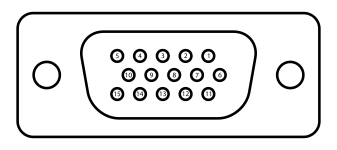
\includegraphics[height=2em]{slides/graphics-hardware/vga-pinout.pdf}
  \end{center}
  \begin{itemize}
  \item \textbf{Pixel}: Red, Green, Blue {\footnotesize(1, 2, 3)}, Ground returns {\footnotesize(6, 7, 8)}
  \item \textbf{Sync}: Hsync, Vsync {\footnotesize(13, 14)}
  \item \textbf{Side}: DDC SDA, DDC SCL {\footnotesize(12, 15)}
  \item \textbf{Power}: \(+5~V\) {\footnotesize(9)}, Ground {\footnotesize(10)}
  \end{itemize}
  \end{itemize}

\end{frame}

\begin{frame}{VGA display interface (illustrated)}
  \begin{center}
    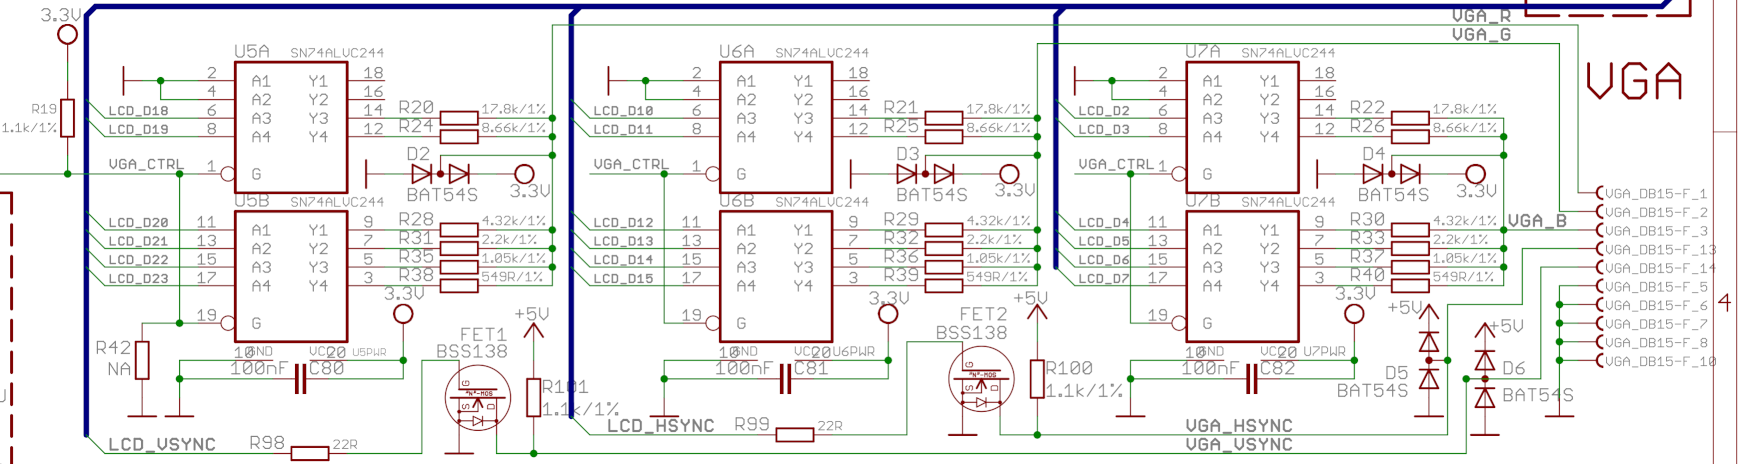
\includegraphics[width=\textwidth]{slides/graphics-hardware/a13-olinuxino-vga.png}
  \end{center}

  \begin{itemize}
  \item Very basic VGA encoder from parallel signals, DDC excluded
  \item Resistor ladder for analog-to-digital conversion\\
  \textit{using SN74ALVC244 voltage level shifters (\(1.8~V\) to \(3.3~V\)), clamping diodes}
  \item 6 most-significant bits only, 2 least-significant bits set to 0\\
  \textit{D0-D1, D8-D9 and D16-D17 are not routed}
  \end{itemize}
\end{frame}

\begin{frame}{DVI display interface}
  \begin{itemize}
  \item \textbf{Digital Visual Interface} (DVI), since 1999 (DDWG)
    \begin{itemize}
    \item \textbf{DVI-A}: Analog only, comparable to VGA
    \item \textbf{DVI-D}: Digital only, single-link (3 data lanes) or dual-link (6 data lanes)
    \item \textbf{DVI-I}: Both analog and digital supported, single-link or dual-link
    \item Digital serial link using \textbf{Transition-Minimized Differential Signaling} (TMDS)
    \item Dedicated \textbf{DDC} and \textbf{HPD} signals
    \item Using a subset or variation of the full \textbf{DVI-I connector} for signals:
    \end{itemize}
  \begin{center}
    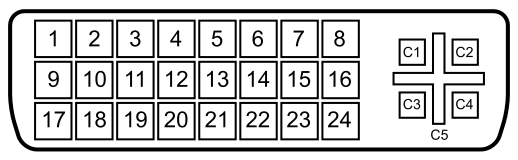
\includegraphics[height=2em]{slides/graphics-hardware/dvi-pinout.pdf}
  \end{center}
  \begin{itemize}
  \item \textbf{TMDS}: Data+ {\footnotesize(2, 5, 10, 13, 18, 21)}, Data- {\footnotesize(1, 4, 9, 12, 17, 20)}, Clock {\footnotesize(23, 24)}
  \item \textbf{Analog pixel}: Red, Green, Blue {\footnotesize(C1, C2, C3)}, Ground {\footnotesize(C5)}
  \item \textbf{Analog sync}: Hsync, Vsync {\footnotesize(C4, 8)}
  \item \textbf{Side}: DDC SDA, DDC SCL {\footnotesize(7, 6)}, HPD {\footnotesize(16)}
  \item \textbf{Power}: \(+5~V\) {\footnotesize(14)}, Ground {\footnotesize(15)}
  \end{itemize}
  \end{itemize}
\end{frame}

\begin{frame}{HDMI display interface}
  \begin{itemize}
  \item \textbf{High-Definition Multimedia Interface} (HDMI), since 2002 (HDMI Forum)
    \begin{itemize}
    \item Similar to \textbf{DVI-D}: no analog, 3 TMDS data lanes (R-G-B)
    \item Adding the use of AVI infoframes for meta-data and audio
    \item \textbf{High bandwidth} \((\leq 48~Gbit/s)\) (2.1) and clock speeds \((\leq 340~MHz)\)
    \item \textbf{Extra features}: Audio, CEC (1.2), HDR (1.3), 4K (1.4), Stereoscopy (1.4),\\8K-10K (2.1), DSC (2.1), HFR (\(120~Hz\)), per-frame HDR (2.1)
    \item Using a dedicated (and proprietary) \textbf{HDMI connector} for signals:
    \end{itemize}
  \begin{center}
    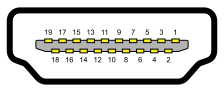
\includegraphics[height=2em]{slides/graphics-hardware/hdmi-pinout.pdf}
  \end{center}
  \begin{itemize}
  \item \textbf{TMDS}: Data+ {\footnotesize(1, 4, 7)}, Data- {\footnotesize(3, 6, 9)}, Clock {\footnotesize(10, 12)}
  \item \textbf{Side}: SDA, SCL {\footnotesize(16, 15)}, HPD {\footnotesize(19)}, CEC {\footnotesize(13)}
  \item \textbf{Power}: \(+5~V\) {\footnotesize(18)}, Ground {\footnotesize(17)}
  \end{itemize}
  \end{itemize}
\end{frame}

\begin{frame}{DP/eDP display interface}
  \begin{itemize}
  \item \textbf{DisplayPort} (DP), since 2008 (VESA)
    \begin{itemize}
    \item Digital serial link with 4 data lanes using \textbf{Low-Voltage Differential Signaling} (LVDS)
    or TMDS for DP Dual-Mode (DP++), compatible with DVI-D and HDMI
    \item Using \textbf{packets} for video/audio data and meta-data 
    \item Auxiliary channel encapsulating I2C DDC, CEC and more (e.g. USB)
    \item \textbf{High bandwidth} \((\leq 77.37~Gbit/s)\) (2.0)
    \item \textbf{Extra features}: Audio, CEC, HDR (1.4), 4K (1.3), Stereoscopy (1.2),\\8K (1.3-1.4),  10K-16K (2.0)
    \item \textbf{Multi-Stream Transport} (MST) to chain displays
    \item Using a dedicated (and proprietary) \textbf{DisplayPort connector} for signals:
    \end{itemize}
  \begin{center}
    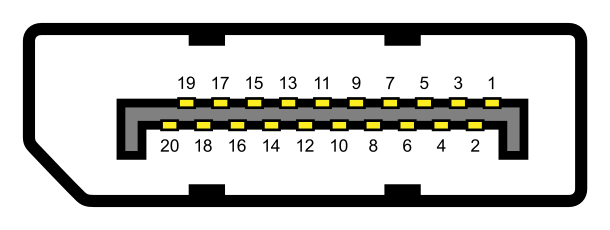
\includegraphics[height=2em]{slides/graphics-hardware/dp-pinout.pdf}
  \end{center}
  \begin{itemize}
  \item \textbf{LVDS/TMDS}: ML+ {\footnotesize(1, 4, 7, 10)}, ML- {\footnotesize(3, 6, 9, 12)}
  \item \textbf{Side}: AUX+ (15), AUX- (17), HPD (18)
  \item \textbf{Power}: \(+3.3~V\) {\footnotesize(20)}, Ground {\footnotesize(2, 5, 8, 11, 16)}
  \end{itemize}
  \item \textbf{Embedded DisplayPort} (eDP) for internal panels (without connector)
  \end{itemize}
\end{frame}

\begin{frame}{LVDS and DSI display interfaces}

% TODO split and add photo of custom LVDS connector as well as a DSI panel (librem 5 dvt?)

  \begin{itemize}
  \item \textbf{Low Voltage Differential Signaling} (LVDS)
    \begin{itemize}
    \item Generic digital serial link with clock and data signals using LVDS
    \item Only sends pixel data according to a pre-defined mode (no DDC, no packets)
    \item For internal panels, exposed with specific connectors
    \item Common for laptop panels
    \end{itemize}
  \end{itemize}
  \begin{itemize}
  \item \textbf{Display Serial Interface} (DSI), since 2006 (MIPI)
    \begin{itemize}
    \item Digital serial link with clock and up to 4 data lanes using LVDS
    \item Using \textbf{packets} for video data and meta-data
    \item Commands for configuration can be issued with the \textbf{DSI Command Set} (DCS)\\
    \textit{Generic base with proprietary vendor-specific extensions}
    \item For internal panels, exposed with specific connectors
    \item Common for mobile devices' panels
    \end{itemize}
  \end{itemize}
\end{frame}

\begin{frame}{DPI display interface}
  \begin{itemize}
  \item \textbf{Display Parallel Interface} (DPI)
    \begin{itemize}
    \item Generic parallel digital interface, with 1 signal per color bit, clock and sync
    \item Exists with different numbers of bits: 24 (8-8-8), 18 (6-6-6) or 16 (5-6-5)\\
    \textit{Dithering is required when using 16 or 18 bits}
    \item Sends pixel data bits following mode timings
    \item Base signals: color data bits, vsync, hsync
    \item Extra signals: display enable (DE)
    \item Beware: sync and DE signals can be active-high or active-low
    \item For internal panels, requires many signals
    \end{itemize}
  \end{itemize}
\end{frame}

\begin{frame}{Bridges/transcoders}
  \begin{itemize}
  \item Not every display interface is supported by the hardware at hand
  \item Bridges or transcoders are used to translate from one interface to another
  \item They are composed of a decoder and an encoder (in a single package)
  \item Usually standalone and transparent, often only replicate timings\\
  \textit{but some can have a side-bus for configuration and fine-tuning}
  \item Example: VGA interfaces are usually bridged from digital interfaces nowadays
  \end{itemize}

  \begin{center}
  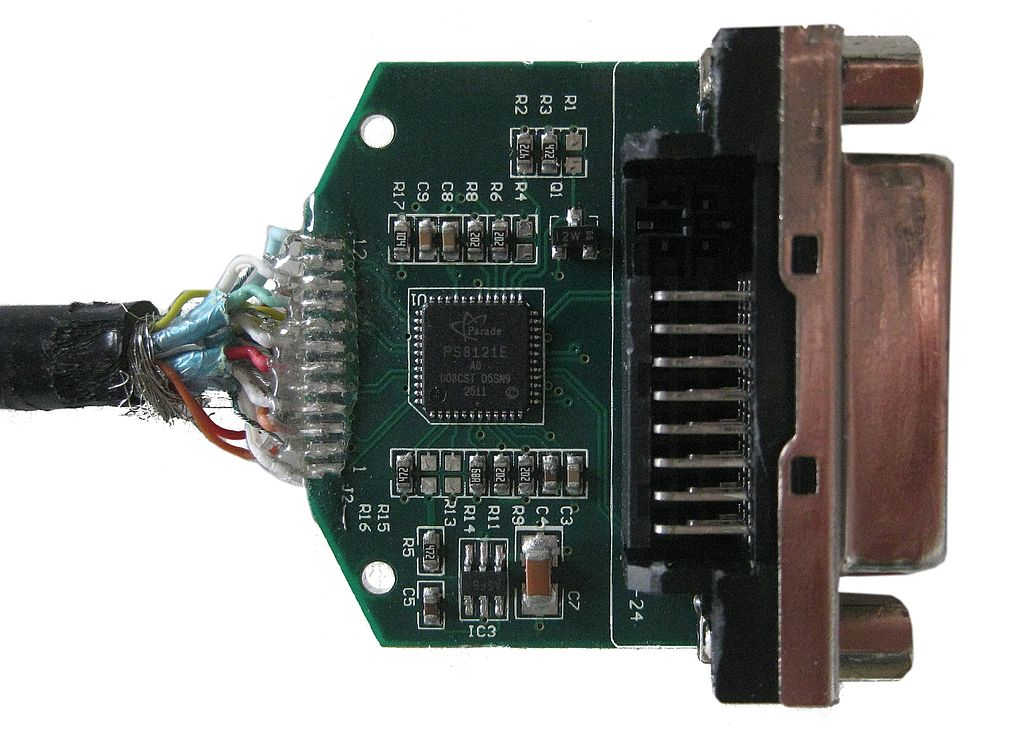
\includegraphics[height=6em]{slides/graphics-hardware/dp-dvi-bridge.jpg}\\
  \textit{\small A DP to DVI bridge}
  \end{center}
\end{frame}

\subsection{Render Hardware Specifics}

\begin{frame}{Digital Signal Processors}
  \begin{itemize}
  \item Digital Signal Processors (DSPs) allow programmable image signal processing\\
    \textit{can also be used for implementing 2D rendering primitives}
  \item Using a dedicated Instruction Set Architectures (ISA)
  \item Arithmetic implementations are either:
    \begin{itemize}
    \item \textbf{fixed-point}: simple hardware implementation, fixed range (usually 16.16)\\
      \textit{16 bits for the integer part and 16 bits for the decimal part}
    \item \textbf{floating-point}: complex implementations, trade-off between range and precision
    \end{itemize}
  \item Usually more power-efficient than general-purpose CPUs
  \item Depending on the DSP, the software can be:
    \begin{itemize}
    \item A \textbf{standalone firmware}, usually developed from vendor libraries (C/C++/ASM)
    \item A \textbf{real-time operating system} (RTOS) application (C/C++/...)
    \end{itemize}
  \item Can be used standalone in a video pipeline or to offload a CPU
  \item Modern DSPs can be multi-core and feature various I/O controllers
  \end{itemize}
\end{frame}

\begin{frame}{Dedicated hardware accelerators}
  \begin{itemize}
  \item Fixed-function hardware can be used for accelerating specific operations
  \begin{itemize}
    \item Implemented as hardware circuits in Systems on a Chip (SoCs) or DSPs
    \item Implemented as logic configuration bitstream in FPGAs
  \end{itemize}
  \item Implement a configurable fixed pipeline for image operations
  \item Accessed and configured through specific registers exposed via a bus
    \begin{itemize}
    \item Global configuration registers to build the pipeline between blocks
    \item Configuration registers for each block
    \item Kick and status registers
    \end{itemize}
  \item Usually very power-efficient and very fast
  \end{itemize}
\end{frame}

\begin{frame}{Dedicated hardware accelerators (illustrated)}
  \begin{center}
    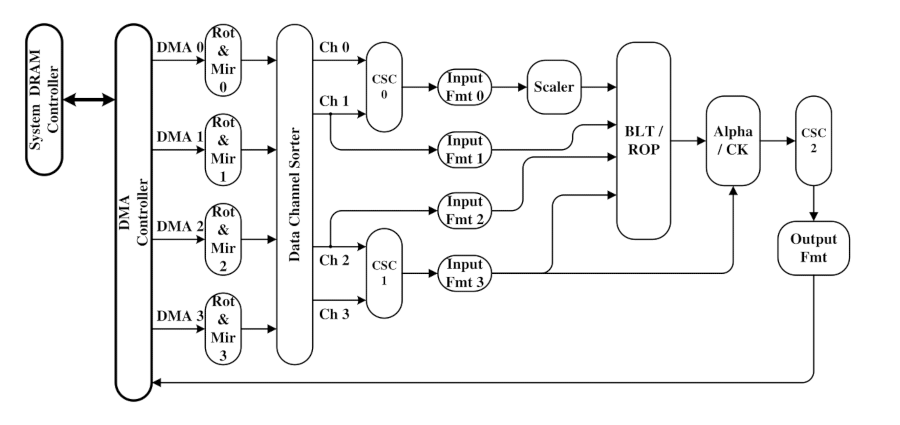
\includegraphics[width=0.7\textwidth]{slides/graphics-hardware/g2d-block.png}\\
    \textit{An example hardware pipeline for a 2D graphics block}\\
  \end{center}
\end{frame}

\begin{frame}{Graphics Processing Unit}
  \begin{itemize}
  \item Graphics Processing Units (GPUs) are \textbf{3D rendering hardware} implementations\\
    \textit{the term no longer designates all graphics-processing hardware}
  \item Operate on 3D graphics primitives: \textbf{points (vertices), lines and triangles}
  \item Generate a 2D view (viewport) from a given perspective
    \begin{itemize}
      \item Objects are formed of interconnected triangles
      \item A color can be applied to each vertex and interpolated
      \item Textures can be applied to objects with texture element to vertex mapping
      \item Lighting is applied from various sources
    \end{itemize}
  \item Expected to render at \textbf{display scanout rate} (pseudo real-time)
    \begin{itemize}
    \item Usually not photo-realistic methods as ray tracing or photon mapping
    \item Extremely efficient compared to any general-purpose CPU
    \end{itemize}
  \item GPUs are also used for general-purpose computing with GPGPU
  \end{itemize}
\end{frame}

\begin{frame}{Graphics Processing Unit architectures}
  \begin{itemize}
  \item GPUs implement a pipeline of hacks accumulated since the 1970s
  \item GPU hardware architectures evolved over time:
    \begin{itemize}
    \item From \textbf{fixed-function} configurable hardware block pipelines
    \item To pipelines with both fixed blocks and specialized \textbf{programmable} processing units
    \end{itemize}
  \item Shaders are programs that run at different steps of the pipeline:
    \begin{itemize}
    \item \textbf{vertex shaders}: define the position, texture coordinates and lighting of each vertex
    \item \textbf{geometry shaders}: generate new primitives from the provided ones
    \item \textbf{tesselation shaders}: perform vertex sub-division (e.g. Catmull-Clark)
    \item \textbf{fragment/pixel shaders}: perform rasterisation for each output pixel
    \end{itemize}
  \item Scenes can be rendered with multiples passes and multiple shaders
  \end{itemize}
\end{frame}

\begin{frame}{Graphics Processing Unit architectures (illustrated)}
  \begin{center}
  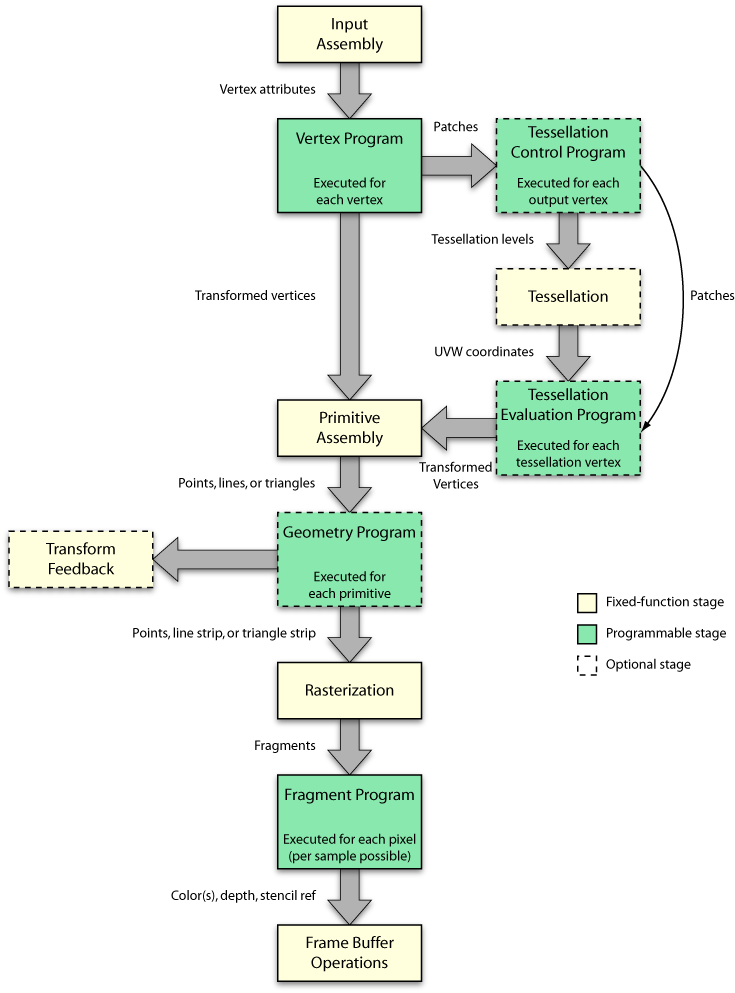
\includegraphics[width=0.5\textwidth]{slides/graphics-hardware/gpu-pipeline.png}\\
  \textit{\small A programmable GPU pipeline}
  \end{center}
\end{frame}

\begin{frame}{Graphics Processing Unit techniques}
  \begin{itemize}
  \item GPUs are optimized for \textbf{performance} and \textbf{good-looking results}
  \item \textbf{Texture sampling} can easily cause aliasing (at a distance)
    \begin{itemize}
    \item \textbf{Bilinear and trilinear filtering} is often used
    \item \textbf{Anisotropic filtering} provides best visual results
    \item \textbf{Mip-maps} provide the same texture at different sizes
    \item \textbf{Multi-Sample Anti-Aliasing} (MSAA) averages colors from multiple points
    \end{itemize}
  \item \textbf{Texture compression} reduces memory pressure (e.g. S3TC, ASTC)
  \item \textbf{Normals mapping/bump maps} provide increased details with low vertex count\\
    \textit{affects light path calculation}
  \item Avoiding \textbf{useless rendering} operations:
    \begin{itemize}
    \item Occluded surfaces are not rendered (visible surface determination)
    \item Using a \textbf{depth/z-buffer} to keep track of the z-order for each output pixel
    \item Culling for early vertex removal: back-face, view frustum, z-buffer
    \end{itemize}
  \end{itemize}
\end{frame}

\begin{frame}{Graphics Processing Unit techniques (illustrated)}
  \begin{minipage}{0.45\textwidth}
    \centering
    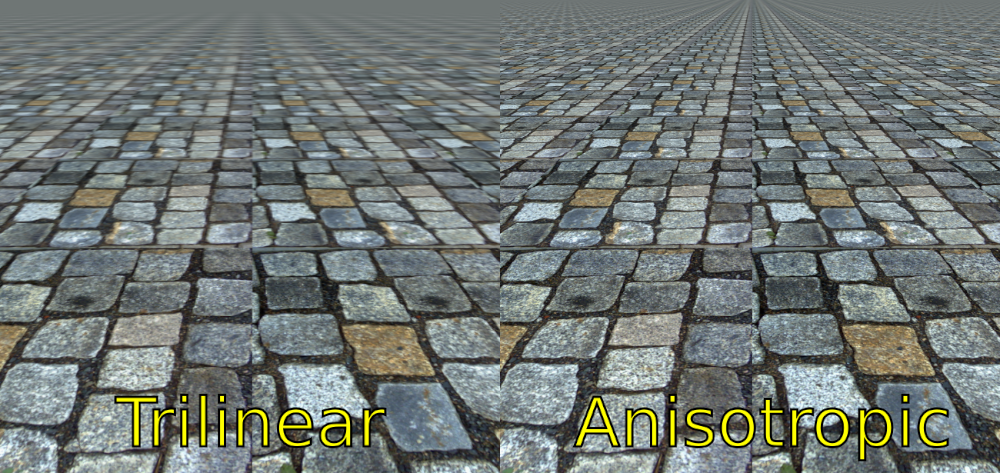
\includegraphics[width=\textwidth]{slides/graphics-hardware/anisotropic-filtering.png}\\
    \textit{Comparison of tri-linear and anisotropic anti-aliasing filtering}
  \end{minipage}
  \hfill
  \begin{minipage}{0.45\textwidth}
    \centering
    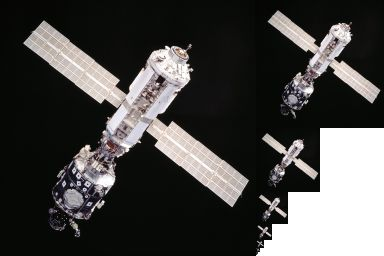
\includegraphics[height=7em]{slides/graphics-hardware/mip-map.jpg}\\
    \textit{A mip-mapped texture representation}
  \end{minipage}
\end{frame}

\begin{frame}{Graphics Processing Unit internals}
  \begin{itemize}
  \item A \textbf{command stream} is parsed and used to configure the pipeline
  \item Shader cores have highly-specialized ISAs adapted for geometry:
  \begin{minipage}[b]{0.45\textwidth}
    \begin{itemize}
    \item Vector operations, SIMD
    \item Trigonometric operations
    \end{itemize}
  \end{minipage}
  \begin{minipage}[b]{0.45\textwidth}
    \begin{itemize}
    \item Interpolation operations
    \item Usually few conditionals
    \end{itemize}
  \end{minipage}
  \item Texture access is provided by a \textbf{Texture Mapping Unit} (TMU)
    \begin{itemize}
    \item Caching is used to reduce memory pressure
    \end{itemize}
  \item Modern GPUs sometimes have a \textbf{unified shader core}\\
    \textit{allows efficient hardware ressources usage, with complex scheduling}
  \item Shading cores are \textbf{duplicated} and work in parallel (especially rasterization)
  \item Some architectures implement tiled processing:
    \begin{itemize}
    \item Output is divided in tiles (clipping areas) and distributed to cores
    \item Each rasterized tile is written to the output framebuffer separately
    \end{itemize}
  \end{itemize}
\end{frame}

\subsection{System Integration, Memory and Performance}

\begin{frame}{Graphics integration and memory}
  \begin{itemize}
  \item Graphics devices integrated in larger systems need two main interfaces:
    \begin{itemize}
    \item \textbf{Control interface} (low speed): to program the device from the main CPU
    \item \textbf{Memory interface} (high speed): to read the source data and write their framebuffer
    \end{itemize}
  \item Other usual required elements: clocks, interrupts, reset
  \item Both the graphics device and the CPU need to access the memory
  \item Different types of memory used by graphics hardware:
    \begin{itemize}
    \item \textbf{graphics memory}: dedicated memory attached to the graphics device\\
    \textit{the memory is made available to the CPU through the memory interface}
    \item \textbf{dedicated system memory}: a reserved contiguous area of system memory\\
    \textit{required when the device has no mapping unit}
    \item \textbf{system memory pages}: any system memory page can be mapped for access\\
    \textit{for devices with a dedicated IOMMU and graphics address remapping table (GART)}
    \end{itemize}
  \item Since the two parties access the same memory, cache can become incoherent
  \item Cache must be \textbf{synchronized} before reading and after writing, or \textbf{disabled}
  \end{itemize}
\end{frame}

\begin{frame}{Shared graphics memory access}
  \begin{itemize}
  \item Concurrent access to memory can lead to trouble:
    \begin{itemize}
    \item Concurrent read-write accesses result in partially-updated data
    \item Concurrent write-write accesses result in incoherent data
    \end{itemize}
  \item Common issue with display hardware: tearing
    \begin{itemize}
    \item The framebuffer is scanned out at a fixed rate (e.g. \(60~fps\))
    \item Any modification during scan out will result in a \textbf{partial update}
    \item Causes an unpleasant \textbf{visual glitch} effect
    \end{itemize}
  \item Solved using (at least) \textbf{double-buffering}:
    \begin{itemize}
    \item The displayed buffer (\textbf{front buffer}) is kept intact
    \item Another buffer (\textbf{back buffer}) is used for drawing the next contents
    \item Front and back buffer are exchanged with \textbf{page flipping}, during vertical blanking
    \item Using more buffers is possible if rendering can be done in advance
    \end{itemize}
  \end{itemize}
\end{frame}

\begin{frame}{Graphics shared memory access (illustrated tearing)}
  \begin{center}
  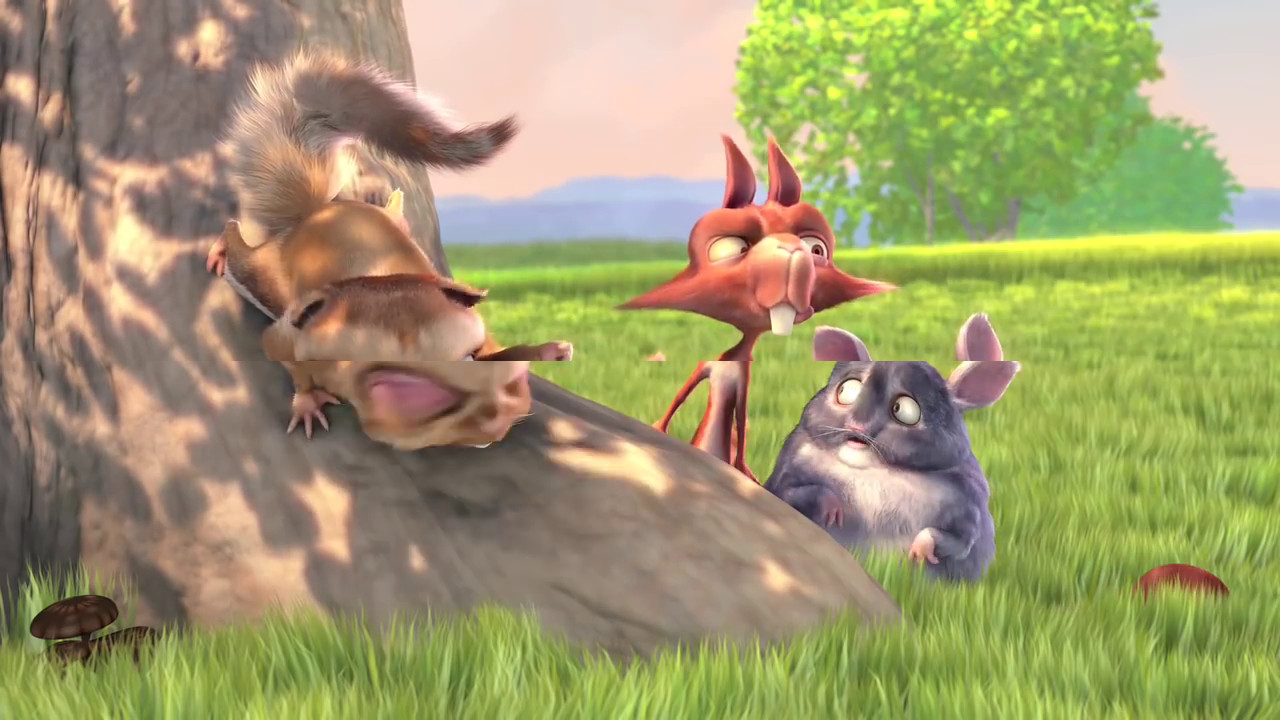
\includegraphics[width=0.7\textwidth]{slides/graphics-hardware/tearing-glitch.jpg}\\
  \textit{\small Tearing example: data is updated during scanout}
  \end{center}
\end{frame}

\begin{frame}{Graphics memory constraints and performance}
  \begin{itemize}
  \item Fixed-pipeline 2D graphics hardware usually streams pixels through FIFOs
  \item A DMA engine fetches pixel data from framebuffer memory
  \item To simplify the logic and optimize memory access, memory constraints may apply:\\
    \begin{itemize}
    \item The start address of each line needs to be aligned to \(2^n\)
    \item The byte size of each line needs to be aligned to \(2^n\)
    \end{itemize}
  \item The \textbf{stride} or \textbf{pitch} describes the line byte size
    \begin{itemize}
    \item Calculated as: \(ALIGN(width \times bpp / 8,~2^n)\)
    \item The size of a framebuffer becomes (single-planar): \(stride \times height\)\\
      \textit{memory may be over-allocated to satisfy alignment constraints}
    \end{itemize}
  \item Pixel order in memory may not follow raster order:
    \begin{itemize}
    \item Optimized depending on the hardware architecture
    \item Optimized for efficient memory access
    \item Tiled orders are frequent for parallel hardware
    \item Framebuffer sizes are calculated with a specific formula
    \end{itemize}
  \end{itemize}
\end{frame}

\begin{frame}{Tiled framebuffer format example}
  \begin{minipage}{0.45\textwidth}
    \centering
    \textit{\small The Allwinner VPU tiled format}
  \end{minipage}
  \hfill
  \begin{minipage}{0.45\textwidth}
    \centering
    \vspace{1em}
    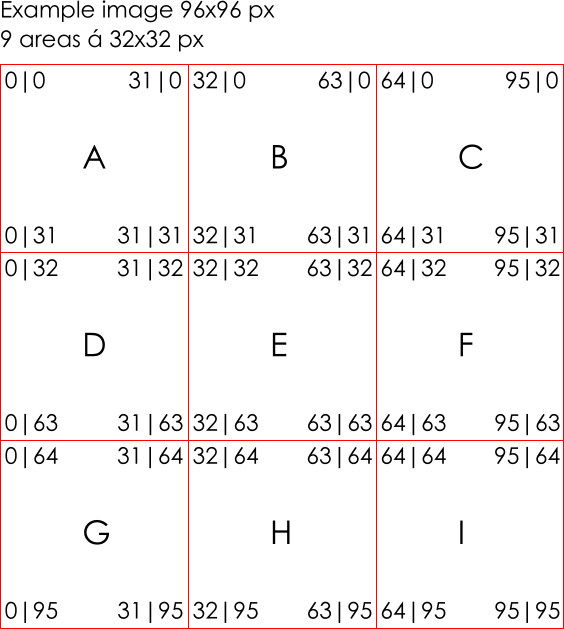
\includegraphics[width=0.35\textwidth]{slides/graphics-hardware/sunxi-tiled-format.png}\\
  \end{minipage}
  \vspace{2em}
  \begin{minipage}[b]{0.45\textwidth}
    \centering
    \vspace{1em}
    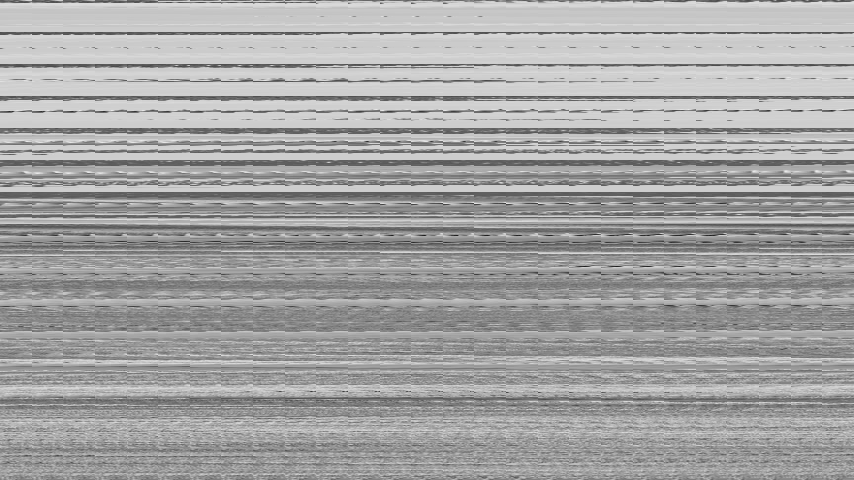
\includegraphics[width=\textwidth]{slides/graphics-hardware/sunxi-tiled-linear.png}
    \textit{\small A tiled framebuffer read in raster order}
  \end{minipage}
  \hfill
  \begin{minipage}[b]{0.45\textwidth}
    \centering
    \vspace{1em}
    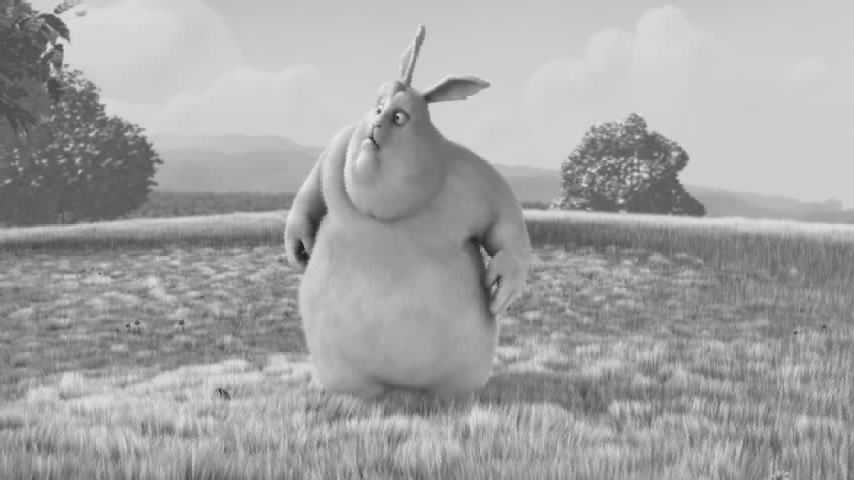
\includegraphics[width=\textwidth]{slides/graphics-hardware/sunxi-tiled.png}
    \textit{\small The same framebuffer read properly}
  \end{minipage}
\end{frame}

\begin{frame}{Offloading graphics to hardware}
  \begin{itemize}
  \item Offloading graphics to hardware liberates significant CPU time
  \item For many use cases, it is crucially needed:
    \begin{itemize}
    \item Video presentation at a given frame-rate, with CSC and scaling
    \item 3D scene rendering at display refresh rate
    \item Windows and cursor composition at display refresh rate
    \end{itemize}
  \item Offloading is not (always) a magical solution:
    \begin{itemize}
    \item Fixed setup costs must be significantly lower than CPU processing time\\
      \textit{small operations are sometimes more efficient on-CPU}
    \item Asynchronous interrupts can introduce latency compared to active polling\\
      \textit{but blocking the whole system is not always an option}
    \end{itemize}
  \item 2D hardware is usually more efficient and adapted than bringing up the GPU\\
    \textit{the GPU is a power-hungry war machine that solves problems at a price}
  \end{itemize}
\end{frame}

\begin{frame}{Graphics performance tips}
  \begin{itemize}
  \item Making the most of hardware can help a lot\\
    \textit{e.g. camera controllers can often provide CSC and scaling}
  \item Generally reducing the number of devices in the graphics pipeline
  \item One major bottleneck in graphics pipelines is memory access:
    \begin{itemize}
    \item Memory buffer copies must be avoided at all costs (zero-copy)
    \item Chained elements in a pipeline should share the same buffer\\
      \textit{hardware constraints are usually compatible in SoCs}
    \end{itemize}
  \item Redrawing full frames should be avoided when possible
    \begin{itemize}
    \item Local operations should be clipped
    \item Buffer damage has to be accumulated in the multi-buffering case
    \end{itemize}
  \item Graphics in operating systems is usually best-effort
  \item DSPs can usually provide real-time guarantees
  \end{itemize}
\end{frame}
